\documentclass[dvipdfmx,autodetect-engine]{jreport}
\usepackage[top=30truemm,bottom=30truemm,left=25truemm,right=25truemm]{geometry}
\usepackage[dvipdfmx]{graphicx}
\usepackage{float}
\usepackage{natbib}

\title{タイコグラフィによる回転体X線結像ミラーのキャラクタリゼーション}
\author{dieu.detruit }
\date{December 2020}

\begin{document}

\begin{center}
\thispagestyle{empty}
{\LARGE 令和2年度 卒業論文}\\
\begin{figure}[H]
    \centering
    
\includegraphics[scale=0.4]{images/utility/utlogo.jpg}
\end{figure}
\vspace*{2.5cm}
{\Huge タイコグラフィ法による}\\
\vspace*{0.5cm}
{\Huge 回転体X線結像ミラーの}\\
\vspace*{0.5cm}
{\Huge キャラクタリゼーション}\\
\vspace*{1.5cm}
{\huge Characterization of Rotation X-ray Imaging Mirror}\\
\vspace*{0.5cm}
{\huge Using Ptychographical Method}\\
\vspace*{3.5cm}
{\LARGE 指導教員 三村 秀和 准教授}\\
\vspace*{1.0cm}
{\Large 東京大学 工学部 精密工学科}\\
{\Large 03-190395}\\
\vspace*{1.0cm}
{\LARGE 渡辺 貴史}
\end{center}

\newpage
\tableofcontents

\newpage
\chapter{序論}
\section{研究の意義・背景}
通常、我々が天体を観測するとき、可視光を通してその形状や特徴を観察する。一方で、天文学では可視光に熱や電磁波、放射線といった可視光以外の物質を通じて様々な現象が明らかにされてきた。中でも、電磁波の一種であるX線を観測することは、天文学において非常に有用である。FOXSI3では太陽コロナを撮影することに成功し、より太陽の構造を明らかにするに至った。ほげほげ

\begin{figure}[h!]
\centering
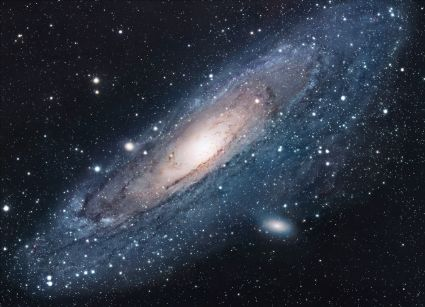
\includegraphics[scale=1.7]{images/utility/universe.jpg}
\caption{The Universe}
\label{fig:universe}
\end{figure}

\section{天文用Wolterミラー}
光を一点に集光するための素子として、屈折を利用するレンズ、反射を利用したミラー、回折を利用したフレネルゾーンプレートなどが有名である。

\section{従来的な直接計測法}

\newpage
\chapter{Wolterミラーの誤差応答シミュレーション}

\newpage
\section{誤差応答シミュレーションの意義}
Wolterミラーを光学系に組み込んで利用する際、大きく分けて2つの誤差によってその理想の集光・結像が損なわれる。ひとつは設計曲面と実際に加工されたミラー表面の形状の誤差、もうひとつはミラー設置時の位置・姿勢の誤差である。
これらを与えたとき集光点の様子がどのようになるか、また集光点の変化として許容できる誤差の範囲はどれほどなのかを見積もることは、Wolterミラー評価の重要な軸となる。6章では、加工されたミラーに対して測定実験を行い、本章で計算した許容誤差との比較・検討を行う。

\section{シミュレーションの方法}
この節では、シミュレーションの方法について述べる。

\section{計算条件}
6章で実際に利用する測定対象のミラーについて、誤差応答のシミュレーションを行う。以下にその設計パラメータを示す。

\section{直径誤差}

\section{扁平誤差}

\section{周方向形状誤差}

\section{長手方向形状誤差}

\section{設置角度誤差}

\section{設置位置誤差}

\newpage
\chapter{Wolterミラー評価実験の手法に関する検討}

\newpage
\section{タイコグラフィ法の概要}
2章でも述べた通り、波面計測は波動光学に基づいており、X線の伝播は複素波動場として与えられる。一方で、CCDカメラなどの撮像素子で得られるのはその振幅の2乗、つまりエネルギーの情報のみである。

\section{焦点面走査による冗長性}
前節で述べた方法について、用いるオブジェクトには大きく分けて2種類ある。1つは透過関数として表現される

\section{疎条件の利用}

\section{ディテクター走査による冗長性}

\section{下流端開口走査による冗長性}

\subsection{対称性}

\newpage
\chapter{レンズによる提案手法の検討}

\newpage

\section{実験の構成}
実験装置の概要を以下に示す。
平行光に対して輪帯状の開口を入れることで、擬似的に輪帯開口の集光光学系を再現する。
輪帯開口の設計

\section{実験の構成}
実験装置の概要を以下に示す。


\newpage
\chapter{結論}
``I always thought something was fundamentally wrong with the universe'' \citep{adams1995hitchhiker}

\newpage
\chapter{謝辞}
ありがとうそしてありがとう

\bibliographystyle{plain}
\bibliography{references}
\end{document}
